\chapter{Cascaded Pictorial Structures}\label{sec:CPS}


\section{Introduction}
Pictorial structure models, first proposed by ~\cite{fischler1973ps} and outline in~\secref{ps}, are a popular method for human body pose estimation~\cite{felz05,fergus2005sparse,devacrf,ferrari08,andriluka09}.
The model is a pairwise structured model over pose variables that characterizes 
local appearance properties of parts and geometric part-part interactions.   
The search over the full pose space is linear time in the number of parts when 
the part-part dependencies form a tree.  However,  the individual part 
state spaces are too large (typically hundreds of thousands of states) to allow 
complex appearance models to be evaluated densely.   Most appearance models are 
therefore simple linear filters on edges, color and 
location~\cite{felz05,devacrf,ferrari08,andriluka09}. 

Similarly, because of quadratic state-space complexity, part-part relationships 
are typically restricted to be image-independent deformation costs that allow 
for convolution or distance transform tricks to speed up 
inference~\cite{felz05}, see~\secref{ps}. A common problem in such models is 
poor localization of parts that have weak appearance cues or are easily 
confused with background clutter (accuracy for lower arms in human figures is 
almost half of that for torso or head~\cite{andriluka09}).   Localizing these 
elusive parts requires richer models of individual part shape and joint 
part-part appearance, including contour continuation and segmentation cues, 
which are prohibitive to compute densely.

In order to enable richer appearance models, we propose to learn a cascade of 
pictorial structures (\CPS) of increasing pose resolution which 
progressively filter the pose state space.  Conceptually, the idea is similar 
to the work on cascades for face detection~\cite{geman2001,viola02}, but the 
key difference is the use of structured models. Each level of the cascade at a 
given spatial/angular resolution refines the set of candidates from the 
previous level and then runs inference to determine which poses to filter out.  
For each part, the model selects poses with the largest {\em max-marginal}
scores, subject to a computational budget.  Unlike conventional pruning 
heuristics, where the possible part locations are identified using the output 
of a detector, models in our cascade use inference in simpler structured models 
to identify what to prune, taking into account global pose in filtering 
decisions.
\begin{figure}[t]
\begin{center}
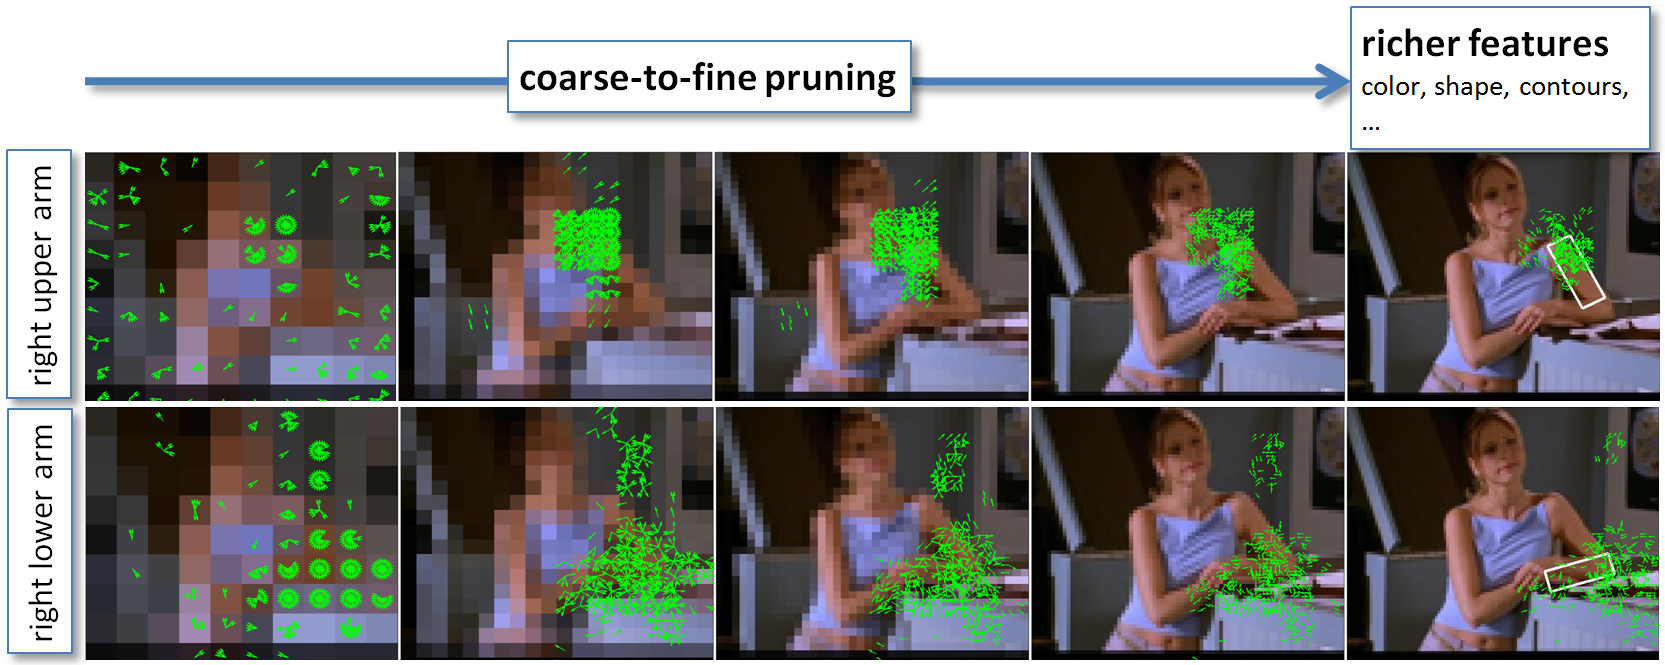
\includegraphics[width=1.0\textwidth]{figs/cps-overview.png}
\end{center}
\caption[Overview of Cascaded Pictorial Structures 
(CPS)]{\label{fig:cps-overview} Overview of CPS:  A discriminative 
coarse-to-fine cascade of pictorial structures filters the pose space so that 
expressive and computationally expensive cues can be used in the final 
pictorial structure.  Shown are 5 levels of our coarse-to-fine cascade for the 
right upper and lower arm parts.  Green vectors represent position and angle of 
unpruned states, the downsampled images correspond to the dimensions of the 
respective state space (but {\em not } the resolution at which features are 
computed), and the white rectangles represent classification using our final 
model.}
\end{figure}
As a result, at the final level the \CPS{} model has to deal with a much 
smaller hypothesis set which allows us to use a rich combination of features.  

In addition to the traditional part detectors and geometric features, we are 
able to incorporate object boundary continuity and smoothness, as well as shape 
features, discussed in detail in~\secref{features}. The former features 
represent mid-level and bottom-up cues, while the latter capture shape 
information, which is complementary to the traditional HoG-based part models.  
The approach is illustrated in the overview Figure~\ref{fig:cps-overview}. We 
apply the presented \CPS model combined with the richer set of features on the 
Buffy and PASCAL Stickmen benchmark, improving the state-of-the-art on arm 
localization, as discussed in~\secref{experiments}. 

\label{subsec:our_ps}
We choose instead to model part configurations as a general linear MRF over 
pairwise and unary terms:
\begin{align}
s(x,y)  = \w \cdot \f(x,y) = \sum_{i \in \cV_\tree} \w_i \cdot \f_i(x,y_i)  + 
\sum_{ij \in \cE_\tree} \w_{ij} \cdot \f_{ij}(x,y_i,y_j)
\label{eq:cps}
\end{align}
where $\tree = (\cV_\tree,\cE_\tree)$ defines a tree structured graph of part 
interactions.  The parameters of our model are the pairwise and unary weight 
vectors $\w_{ij}$ and $\w_i$ corresponding to the pairwise and unary feature 
vectors $\f_{ij}(x,y_i,y_j)$ and $\f_i(x,y_i)$.   The key differences with the 
classical PS model are (1) our pairwise costs allow data-dependent terms, and 
(2) we do not constrain our parameters to fit any parametric distribution such 
as a Gaussian distribution, as is done 
in~\citet{felz05,devacrf,andriluka09,eichner09}.  This is strictly more 
general.  For example, we can express the pairwise features used in the 
classical model as $y_{i} \cdot y_{i}$, $y_{j}\cdot y_{j}$, and $y_{i}\cdot 
y_{j}$ without requiring that their corresponding weights can be combined into 
a positive semi-definite covariance matrix.

In this general form (\equref{cps}), inference can {\em not} be performed 
efficiently with distance transforms or convolution as discussed 
in~\secref{dt}, and we rely on standard $O(nk^2)$ dynamic programming 
techniques to compute the best scoring assignment $\argmax_y s(x,y)$.  Many 
highly effective pairwise features one might design would be intractable to 
compute in this manner for a reasonably-sized state space---for example an $80 
\times 80$ spatial grid with a part angle discretization of $24$ bins yields 
$k^2 \approx 1$ billion part-part hypotheses.

In~\secref{SPC}, we describe how we circumvent this issue via a cascade of 
models which aggressively prune the state space at each stage typically without 
discarding the correct sequence.  After the state space is pruned, we are left 
with a small enough number of states to be able to incorporate powerful 
data-dependent pairwise and unary features into our model.


\section{Related work}
For unstructured, binary classification, cascades of classifiers have been 
quite successful for reducing computation.  \citet{geman2001} propose a 
coarse-to-fine sequence of binary tests to detect the presence and pose of 
objects in an image.  The learned sequence of tests is trained to minimize 
expected computational cost.  The extremely popular Viola-Jones 
classifier~\citep{viola02} implements a cascade of boosting ensembles, with 
earlier stages using fewer features to quickly reject large portions of the 
state space.

Our cascade model is inspired by these binary classification cascades. In 
natural language parsing, several works \citep{carreras2008tag,petrov:PhD} use 
a coarse-to-fine idea closely related to ours and~\citet{geman2001}: the 
marginals of a simple context free grammar or dependency model are used to 
prune the parse chart for a more complex grammar.

Recently,~\citet{pff-cascade} proposed a cascade for a structured parts-based 
model.  Their cascade works by early stopping while evaluating individual 
parts, if the combined part scores are less than fixed thresholds.  While the 
form of this cascade can be posed in our more general framework (a cascade of 
models with an increasing number of parts), we differ from~\citet{pff-cascade} 
in that our pruning is based on thresholds that adapt based on inference in 
each test example, and we explicitly learn parameters in order to prune safely 
and efficiently. In~\citet{geman2001,viola02,pff-cascade}, the focus is on 
preserving established levels of accuracy while increasing speed.  The focus in 
this paper is instead developing more complex models---previously infeasible 
due to the original intractable complexity---to improve state-of-the-art 
performance.

A different approach to reduce the intractable number of state hypotheses is to instead propose a small set of likely hypotheses based on bottom-up perceptual grouping principles~\cite{mori04,Srinivasan07}.  Mori et al.~\cite{mori04} use bottom-up saliency cues, for example strength of supporting contours, to generate limb hypotheses.  They then prune via hand-set rules based on part-pair geometry and color consistency. The shape, color and contour based features we use in our last cascade stage are inspired by such bottom-up processes.  However, our cascade is solely a sequence of discriminatively-trained top-down models.



\section{Structured Prediction Cascades} \label{sec:SPC}
The recently introduced Structured Prediction Cascade framework~\cite{cascades} 
provides a principled way to prune the state space of a structured prediction 
problem via a sequence of increasingly complex models.
There are many possible ways of defining a sequence of increasingly complex 
models.  In~\cite{cascades} the authors introduce higher-order cliques into 
their models in successive stages (first unary, then pairwise, ternary, etc.).  
Another option is to start with simple but computationally efficient features, 
and add more complex features downstream as the number of states decreases.  
Yet another option is to geometrically coarsen the original state space and 
successively prune and refine.
 We use a coarse-to-fine state space approach with simple features until we are 
at a reasonably fine enough state space resolution and left with few enough 
states that we can introduce more complex features.  We start with a severely 
coarsened state space and use standard pictorial structures unary detector 
scores and geometric features to perform quick exhaustive inference on the 
coarse state space.  

\subsection{Inference}
\begin{figure}[tb]
\begin{center}
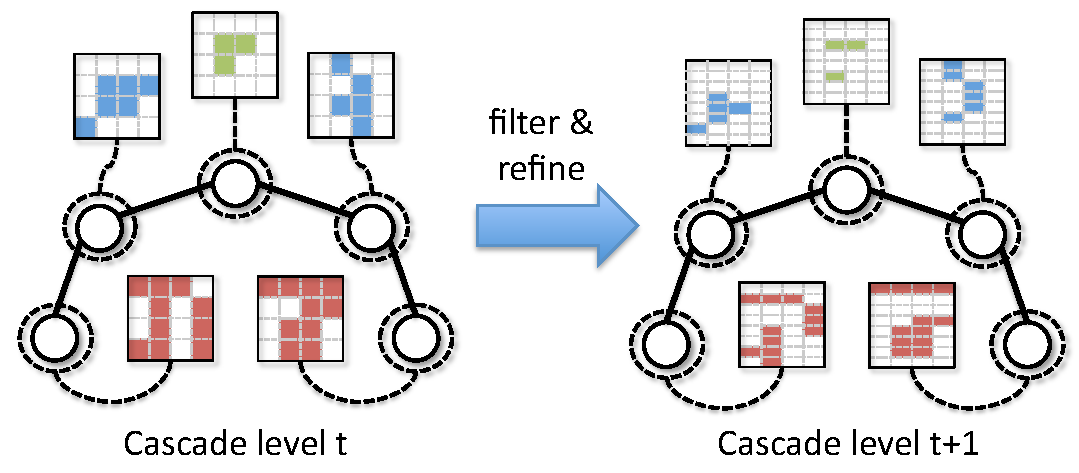
\includegraphics[width=0.99\textwidth]{figs/cascade-concept.pdf}
\caption[Intermediate cascade filtering/refinement step.]{Two consecutive stages of a cascade, showing a model with a sparse set of states in a coarsened state space (top) filtering out states, and then passing them on to the next model (bottom) which works on a finer, upsampled version of the state space.}
\label{fig:cascade-concept}
\end{center}
\end{figure}


The procedure for CPS described above is as follows.  Two intermediate steps of the process are conceptualized in~\figref{cascade-concept}.

\begin{itemize}
\item For an input $x$, initialize a coarse state space $\cS_0 = \cY_0$ by 
spatially pooling states in the original space (downsampling the state space 
volume).

\item Repeat for each cascade level $t = 0,\ldots,T-1$:
\begin{itemize}
\item Run sparse, exact inference over  $\cS_t$ using the $t^{th}$ cascade 
model, computing max-marginal scores.
\item Filter states based on max-marginal scores to obtain $\tilde{\cS}_t$:\\
\indent For each $i$, filter $y_i$ if $\mmi < t_x$, a data-dependent threshold (see~\secref{cps-thresh}).

 \item Refine the state space of $\tilde{\cS}_t$ to obtain $\cS_t$ for 
the next cascaded model.
\end{itemize}
\item Predict using the final level: $y^\star = \argmax_{y \in \cY_T} s(x,y)$.
\end{itemize}


The key ingredient to the cascade framework is that states are pruned using 
{\em max-marginal} scores, introduced in~\secref{max-marginals}, computed 
efficiently using dynamic programming techniques.  The notion of a max-marginal 
is intuitively explained in our model of pose estimation:  The max-marginal for 
a part $i$ at location $y_i$ is the score of the highest scoring pose with part $i$ fixed or ``pinned'' to location $y_i$. Importantly, max-marginals are a {\em 
global} quantity of a complete model of pose, rather than a local one: A part 
could have weak individual image evidence of being at location $y_i$ but still 
have a high max-marginal score if the rest of the model believes this is a 
likely location. 

\subsection{Filtering threshold}\label{sec:cps-thresh}

When applying a cascade, we have two competing objectives that we must trade 
off, accuracy and efficiency: we want to minimize the number of errors incurred 
by each level of the cascade  and maximize the number of filtered 
max-marginals.  A natural strategy is to prune away the lowest ranked states 
based on max-marginal scores. Instead, we prune the states whose max-marginal 
score is lower than a data-specific threshold $t_x$: $y_i$ is pruned if $\mmi < 
t_x$.  This threshold is defined as a convex combination of the highest score
$s^\star_x = \max_y s(x,y)$ and the {\em mean max-marginal score}, defined as:
\begin{equation}
\bar{s}^\star_x = \frac{1}{n} \sum_{i=1}^n \frac{1}{|\cY_i|} \sum_{y_i \in 
\cY_i} \mmi.
\end{equation}
which is just the average $\mmi$ over all parts and all states for each part.  Our thresholding function is thus
\begin{equation}
t_x(s,\alpha) = \alpha s^\star_x + (1-\alpha)\bar{s}^\star_x
\end{equation}
where $\alpha\in[0,1]$ is a parameter to be chosen that 
determines how aggressively to prune. When $\alpha = 1$, only the best state is 
kept, which is equivalent to finding the best, unconstrained assignment.  When $\alpha = 0$ 
approximately half of the states are pruned (if the median of max-marginals is 
equal to the mean).  The reasons for choosing $t_x(s,\alpha)$ are (1) it is a 
function of the image $x$, which allows a threshold that adapts to the 
difficulty of the problem, and (2) it leads to a convex learning formulation 
with additional guarantees, as opposed to sorting max-marginals and choosing a 
cutoff.

\out{
The advantage of using  $t_x(s,\alpha)$ is that it 
is convex in $s(x,y)$, and leads to a convex formulation for parameter 
estimation that trades off the proportion of incorrectly pruned states with the 
proportion of unpruned states.
Note that  $\alpha$ controls efficiency, so we focus on learning the parameters $\theta$ that 
minimize the number of errors for a given filtering level $\alpha$.   
}
\subsection{Learning}
The goal of learning is to fit parameters to our models $\w$ such that they are 
optimized for the task of filtering states efficiently and accurately.  This is 
notably different than standard supervised learning, which attempts to find 
$\w$ to separate the right answer from wrong.  In some sense, the filtering 
learning object is easier to learn---the correct answer does not have to be the 
highest scoring, but only above the threshold value.  To wit, we pose the 
following hard-constraint learning objective, assuming a training set of pairs 
$\{(x^{(j)},y^{(j)})\}_{j=1}^M$:
\begin{align}
\minimize_\w& \frac{1}{2} ||\w||_2^2 \\
\subjectto& s(x^{(j)},y^{(j)}) \geq t_{x^{(j)}}(s,\alpha) + 1,\;\;\; \forall \; j
\end{align}
In words, the above is attempting to find a regularized set of weights $\w$ 
such that, in every training example, the score of the correct pose is above 
our image-adaptive threshold.  We convert the hard constraint objective into an 
unconstrained hinge-loss form typical of a max-margin structured learning 
problem (see~\secref{learning}):
\begin{align}
\minimize_\w& \frac{\lambda}{2} ||\w||_2^2 + \frac{1}{M} \sum_{j=1}^M \left[ 
t_{x^{(j)}}(s,\alpha) - s(x^{(j)},y^{(j)}) + 1 \right]_+
\label{eq:cps-learn-hinge}
\end{align}


The learning formulation uses a simple fact about max-marginals and the 
definition of $t_x(s,\alpha)$
to get a handle on errors of the cascade:
if $s(x,y) > t_x(s,\alpha)$, then for all $i$, $\mmi >  t_x(s,\alpha)$, so no 
part state of $y$ is pruned.   Given an example $(x,y)$,
this condition $s(x,y) > t_x(s,\alpha)$ is {\em sufficient} to ensure that no 
correct part is pruned, which is our justification for using max-marginals as 
the pruning quality.  Note that probabilistic marginals do {\em not} have this 
property: $p(y|x)$ being above a threshold does not guarantee that $p(y_i|x)$ 
are above a threshold for all $i$.

We solve \eqref{eq:cps-learn-hinge} using stochastic
sub-gradient descent. Given an example $(x,y)$, we apply the following when the 
term $\left[ t_x(s,\alpha) - s(x,y) + 1 \right]_+$ (and the sub-gradient) is 
non-zero:
\begin{equation} \label{eq:spf_update}
\w  \leftarrow \w + \eta \left[-\lambda \w + \f(y,x) - \alpha \f(y^\star,x)  - 
(1-\alpha) \bar{\f}^\star(x) \right].
\end{equation}
Above, $\eta$ is a learning rate parameter, $y^\star = \argmax_{y'}
s(x,y')$ is the highest scoring assignment and $\bar{\f}^\star(x)$ are the 
average features used by all max-marginal witnesses $\witnessi $ (explained 
in~\secref{max-marginals}):
\begin{equation}
\bar{\f}^\star(x) = \frac{1}{n} \sum_{i=1}^n \frac{1}{|\cY_i|} \sum_{y_i \in 
\cY_i} \f(x,\witnessi).
\end{equation}
The key distinguishing feature of this update as compared to
structured perceptron is the last term which subtracts features included in all
max-marginal assignments $\witnessi$.

\out{\footnote{Note that because \eqref{eq:convex_opt} is $\lambda$-strongly 
convex,
if we chose $\eta_t = 1/(\lambda t)$ and add a projection step to keep 
$\theta$ in a closed set, the update would correspond to the Pegasos
update with convergence guarantees of $\tilde{O}(1/\epsilon)$ iterations for
$\epsilon$-accurate solutions~\cite{shalev-shwartz07pegasos}.  In our experiments, we found the projection step made no difference and used only 2 passes over the data, with $\eta$ fixed.}.
%, as we discuss in Section~\ref{implementation}.
}

\mypar{Sequential cascade learning} The stages of the cascade are learned 
sequentially, from coarse to fine, and each has a different set of parameters 
$\w$ and $\mathcal{Y}_i$ for each part, as well as $\alpha$.  The states of the 
next level are simply refined versions of the states that have not been pruned.  
We describe the refinement structure of the cascade in~\secref{experiments}.

\out{
In the end of a coarse-to-fine cascade we are left with a small, sparse set of 
states that typically contains the groundtruth states or states relatively 
close to them---in practice we are left with around 500 states per part, and 
95\% of the time we retain a state the is close enough to be considered a match 
(see Table~\ref{tab:pruning}). At this point we have the freedom to add a 
variety of complex unary and pairwise part interaction features involving 
geometry, appearance, and compatibility with perceptual grouping principles 
which we describe in Section~\ref{sec:features}.
}

\subsection{Why not just detector-based pruning?} A \naive approach used in a 
variety of applications is to simply subsample states by thresholding outputs 
of part or sparse feature detectors, possibly combined with non-max 
suppression.  Our approach, based on pruning on max-marginal values in a 
first-order model, is more sophisticated: for articulated parts-based models, 
strong evidence from other parts can keep a part which has weak individual 
evidence, and would be pruned using only detection scores.  The failure of 
pre-filtering  part locations in human pose estimation is also noted 
by~\citet{andriluka09}, and serves as the primary justification for their use 
of the dense classical PS.  This is illustrated in~\figref{cascade-pruning}.

\begin{figure}[tb]
\begin{center}
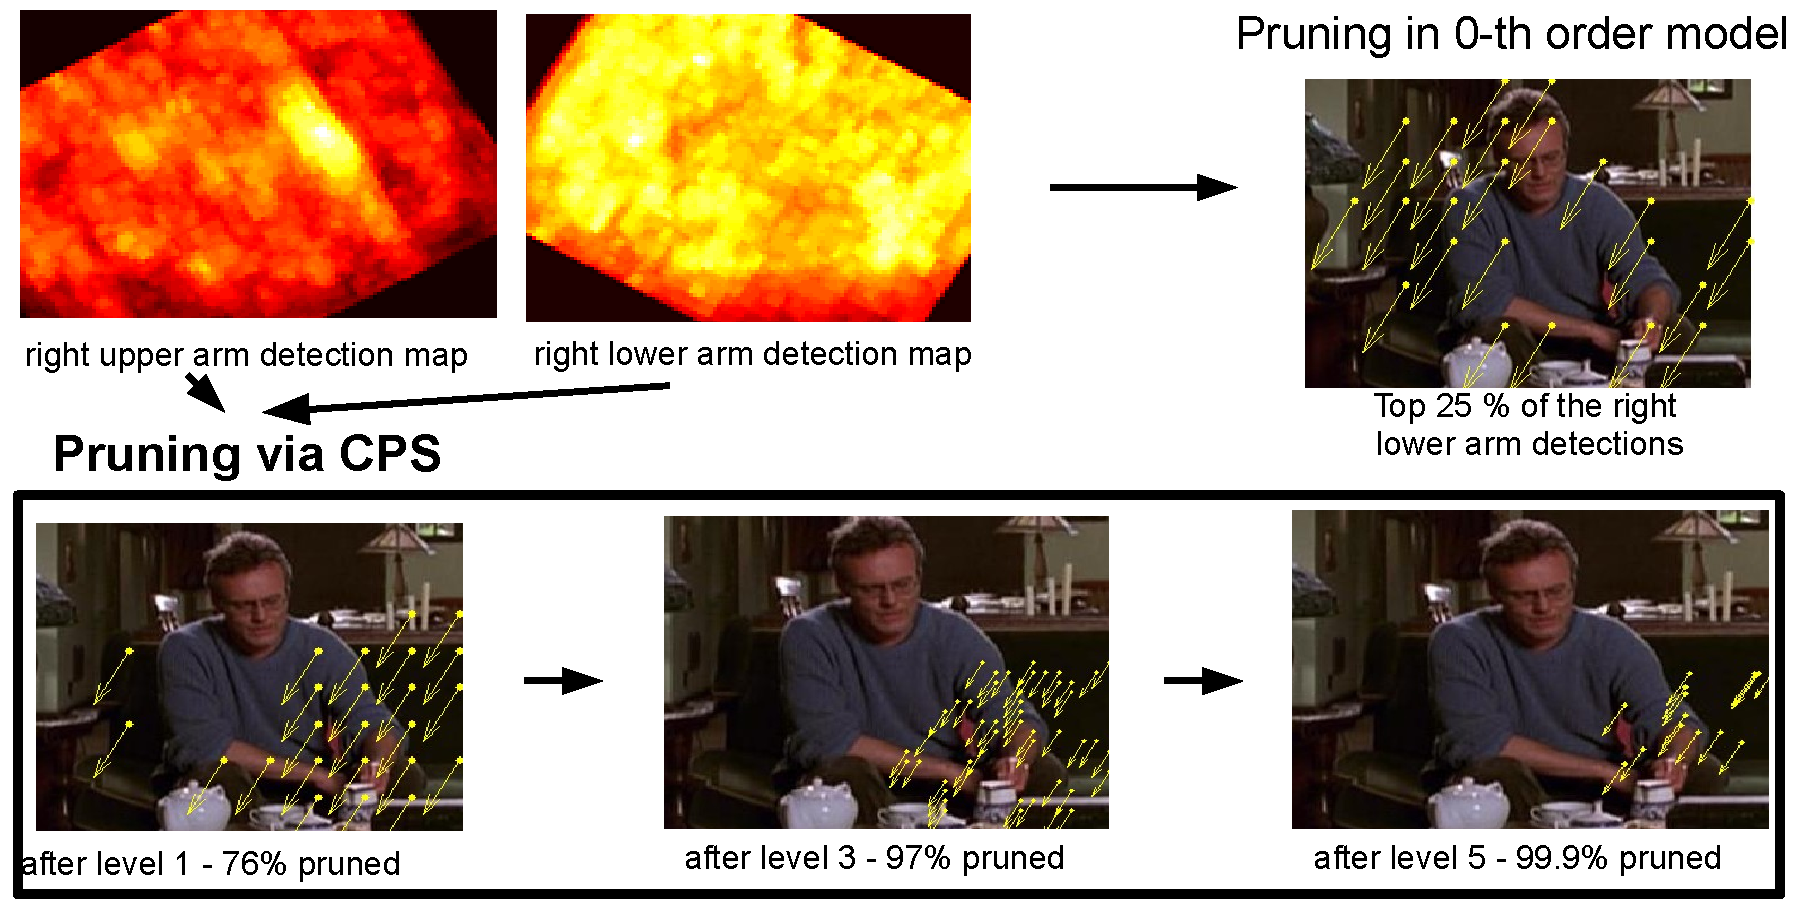
\includegraphics[width=0.99\textwidth]{figs/cascade-pruning.pdf}
\caption[Cascade filtering example]{Cascade filtering example. Detector-based 
pruning (0th order model) by thresholding yields many hypotheses far way from 
the true one for the lower right arm. The CPS (bottom row), however, exploits 
global information (such as certainty of the shoulder location) to perform 
better state pruning.}
\label{fig:cascade-pruning}
\end{center}
\end{figure}




